\section{Anhang}

\subsection{Systemspezifikation}

\begin{figure}
	\centering
	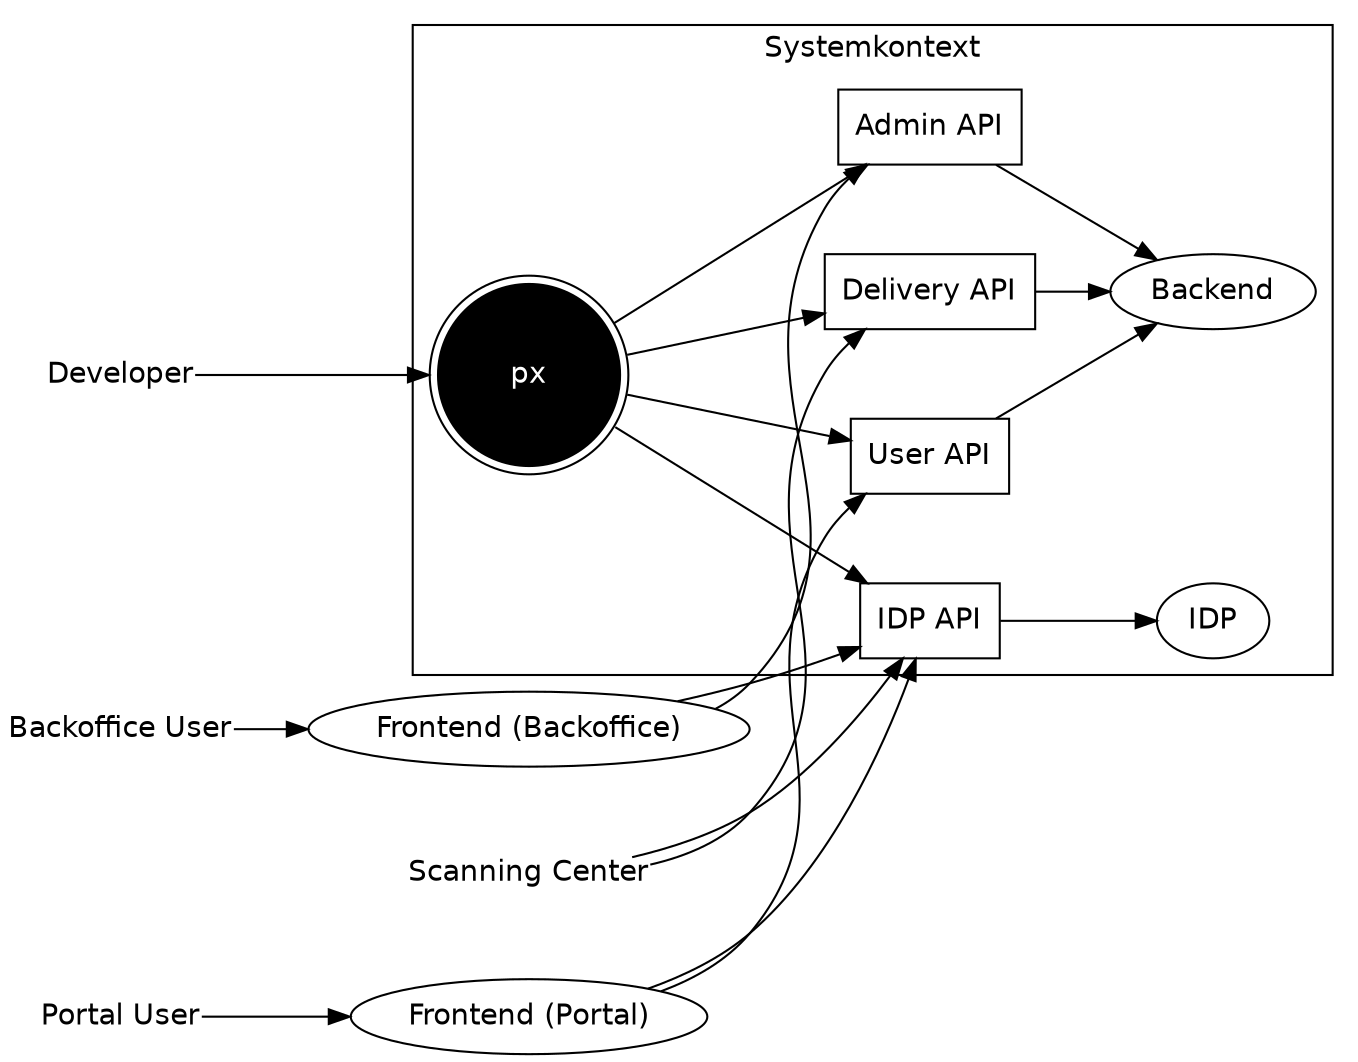
\includegraphics[width=\linewidth]{pics/kontextdiagramm.png}
	\caption{Kontextdiagramm: \texttt{px} als der Gegenstand der Arbeit innerhalb des Systemkontexts}
	\label{fig:kontextdiagramm}
\end{figure}

\subsection{Technologie-Evaluation}

- Vorgabe: PEAX API (RESTful)

\subsubsection{Programmiersprache}

Aus der Aufgabenstellung und dem Umfeld bei PEAX ergeben sich folgende nicht-funktionale Anforderungen an die zu erstellende Software:

\begin{description}
    \item[Installation] Die Software soll sich einfach installieren lassen.
    \item[Umgebung] Es dürfen keine besonderen Anforderungen an die Umgebung gestellt werden, auf der \texttt{px} läuft.
    \item[Plattformen] Die Software soll auf allen gängigen, d.h. bei PEAX eingesetzten, Betriebssystemen (Windows, mac OS, Linux) lauffähig sein.
    \item[Einheitlichkeit] Der Client soll überall die gleiche Befehlssyntax haben.
    \item[Performance] Ein Command Line Client soll in Skripten verwendet werden können, wodurch das Programm sehr oft in kurzem Zeitraum aufgestartet werden muss.
\end{description}

Java, das bei PEAX im Backend-Bereich zum Einsatz kommt, erfordert die lokale Installation einer JRE in der richtigen Version, was bei Frontend-Entwicklern nicht gegeben ist. Ausserdem werden Wrapper-Skripts benötigt (\texttt{java -jar px.jar} ist nicht praktikabel).

Python, Ruby, Perl und andere Skriptsprachen benötigen ebenfalls einen vorinstallierten Interpreter in der richtigen Version.

Zwar gibt es mit Mono eine Variante von .Net, die überall lauffähig ist, hier werden aber wiederum eine Laufzeitumgebung bzw. vorinstallierte Libraries benötigt.

Für die Problemstellung am besten geeignet sind kompilierte Sprachen (C, C++, Go, Rust, Nim). Mit einer statischen Kompilierung lässt sich das ganze Programm in eine einzige Binärdatei überführen, welches denkbar einfach zu installieren ist (Kopieren nach einem der Verzeichnisse innerhalb von \texttt{\$PATH}).

Für JavaScript, das bei PEAX im Frontend zum Einsatz kommt, gibt es mit QuickJS\footnote{\url{https://bellard.org/quickjs/}} seit kurzem die Möglichkeit, JavaScript zu Binärdateien zu kompilieren. Dies funktioniert aber nicht auf allen Plattformen, ausserdem ist QuickJS noch experminentell und noch nicht für den produktiven Einsatz geeignet.

Um ein Projekt vom gegebenen Umfang innerhalb eines Semesters umsetzen zu können, sind Vorkenntnisse in der einzusetzenden Programmiersprache zwar nicht zwingend, können das Risiko des Scheiterns aber erheblich senken. Gerade bei der Abschätzung von Aufwänden ist Vertrautheit mit den einzusetzenden Werkzeugen sehr hilfreich.

Was (statisch) kompilierte Programmiersprachen betrifft, konnte der Autor dieser Arbeit bereits Erfahrungen mit C, Go und Rust sammeln. Das manuelle Speichermanagement in C (u.a. auch bei Strings) ist einerseits ein grosses Risiko (Buffer Overflows, Segmentation Faults), und wirkt sich andererseits negativ auf das Entwicklungstempo aus. In die engere Auswahl kommen somit Go und Rust.

Im Folgenden werden die gemachten Erfahrungen und die dabei empfundenen Vor- und Nachteile mit den Programmiersprachen Go und Rust einander gegenübergestellt.

\subsubsection{Go}

Mit Go konnte der Autor dieser Arbeit bereits einges an Erfahrung sammeln. So wurde neben dem Prototyp zu \texttt{px} bereits die Testat-Aufgabe im Modul Software Testing\footnote{\url{https://github.com/patrickbucher/getting-to-philosophy}}, ein Thumbnailer\footnote{\url{https://github.com/patrickbucher/thumbnailer}} sowie zahlreiche Utilities\footnote{\url{https://github.com/patrickbucher/go-scratch}} (viele darunter als HTTP-Clients) in Go entwickelt. Dabei wurden folgende Vor- und Nachteile ermittelt:

\begin{itemize}
	\item Vorteile
		\begin{itemize}
			\item aufgrund weniger Keywords und Features einfach zu lernen
			\item hervorragendes Tooling out-of-the-box
			\item Cross-Compilation ohne Zusatztools auf alle unterstützte Plattformen möglich
			\item schnelle Kompilierung
			\item umfassende Standard-Library, die u.a. ein hervorrangendes HTTP-Package beinhaltet
			\item persönlich bereits viel (positive) Erfahrungen damit gesammelt
			\item wird bereits für andere bei PEAX gebräuchliche CLI-Tools eingesetzt (\texttt{oc}, \texttt{docker})
			\item fügt sich sehr gut in die UNIX-Philosophie ein (Tooling, Libraries)
			\item Einfaches Interface für nebenläufige Programmierung (Goroutines und Channels)
			\item geringer Memory-Verbrach bei relativ hoher Performance\footnote{\url{https://benchmarksgame-team.pages.debian.net/benchmarksgame/fastest/go.html}}
		\end{itemize}
	\item Nachteile
		\begin{itemize}
			\item fehlende Features wie Generics und \texttt{filter}/\texttt{map}/\texttt{reduce}
			\item Binaries fallen relativ gross aus\footnote{\url{https://golang.org/doc/faq\#Why\_is\_my\_trivial\_program\_such\_a\_large\_binary}}
			\item Error-Handling aufwändig und teils repetitiv
		\end{itemize}
\end{itemize}

\subsubsection{Rust}

Der Autor dieser Arbeit konnte sich bereits letztes Jahr im Rahmen des Moduls \textit{Programming Concepts and Paradigms} an der HSLU Informatik mit Rust befassen \cite[p. 12]{pcp-rust}. Nach selbständiger Beschäftigung mit dieser Programmiersprache im Sommer können (teils ergänzend) folgende Vor- und Nachteile genannt werden:

\begin{itemize}
	\item Vorteile
		\begin{itemize}
			\item viele moderne Features (Generics, \texttt{filter}/\texttt{map}/\texttt{reduce})
			\item hervorragendes Typsystem
			\item gutes und ausgereiftes Tooling
			\item weder manuelles Memory-Management noch Garbage Collector nötig
			\item Pattern Matching führt zu sehr solidem Code
			\item gegenüber Go schlankere Binaries
			\item kommt bereits in der Form einiger CLI-Tools persönlich zum Einsatz (\texttt{rg}, \texttt{bat}, \texttt{hexyl}, \texttt{battop})
			\item erstklassige Performance (im Bereich von C/C++) bei geringem Speicherverbrauch\footnote{\url{https://benchmarksgame-team.pages.debian.net/benchmarksgame/fastest/rust-go.html}}
		\end{itemize}
	\item Nachteile
		\begin{itemize}
			\item hohe Einstiegshürde und lange Einarbeitungszeit
			\item Cross-Compilation benötigt Zusatztools
			\item noch keine praxisnahe Erfahrung damit gesammelt
			\item aufgrund schlanker Standard Library auf viele Dependencies angewiesen
		\end{itemize}
\end{itemize}

\subsubsection{Entscheidung}

Rust hat gegenüber Go einige unbestreitbare Vorzüge (Memory Management, Typsystem, Ausdrucksstärke, Eliminierung ganzer Fehlerklassen, Performance, schlankere Binärdateien). Bezogen auf das umzusetzende Projekt fallen jedoch einige davon kaum ins Gewicht (etwa Performance und Zero-Cost Abstractions). Hier fallen die Vorzüge von Go (umfassende Standard Library, Cross-Compilation) wesentlich stärker ins Gewicht.

Gerade die absichtlich schlank gehaltene Standard Library von Rust, die etwa zur Generierung von Zufallszahlen bereits externe Abhängigkeiten erfordert\footnote{\url{https://doc.rust-lang.org/book/ch02-00-guessing-game-tutorial.html\#using-a-crate-to-get-more-functionality}}, dürfte sich im vorliegenden Projektrahmen negativ auswirken, zumal die Evaluation verschiedener Libraries einen sehr hohen Zusatzaufwand zur Folge haben.

Da Go bereits bei der Entwicklung des Prototypen von \texttt{px} erfolgreich zum Einsatz kam, und einige Projektaspekte (grundlegende CI-Pipeline, \texttt{Makefile} für Cross-Compilation und Packaging) bereits damit implementiert werden konnten, soll Go für das vorliegende Projekt den Vorzug erhalten.

Eine spätere Neuimplementierung von \texttt{px} in Rust wäre ein technisch durchaus interessantes, wenn auch praktisch wenig dringendes ‒ als Fallstudie aber durchaus lohnendes ‒ Unterfangen.

\subsection{Libraries}

TODO: JWT, Keystore, Password Input
